\documentclass[12pt]{article}
   
   \usepackage[utf8]{inputenc}
   \usepackage{graphicx}
   \usepackage{float}
   \usepackage{subcaption}
   %\usepackage{mathtools}
   \usepackage{amsmath}
   
   \addtolength{\hoffset}{-0.7in}
   \addtolength{\textheight}{1.5in}
   \addtolength{\textwidth}{1.5in}
   \addtolength{\voffset}{-1in}
 
\title{EE 214: Experiment - 1 \\
       Characterization of CMOS Transistor}
       
\author{Hitesh Kandala, 180070023 }
\date{January 25, 2020}

\begin{document}
 \maketitle

  \section{Overview of the Experiment and Setup:}
  
  In this experiment we characterized a CMOS inverter. To characterize a CMOS inverter, we have done a DC (or steady state behaviour) characterization by measuring its transfer characteristics and output characteristics and also an AC (or transient behaviour) characterization and measured the inverter delay and its dependence on the power supply, and observed the currents drawn from the power supply.
  
  \begin{itemize}
      \item For measuring the characteristics, we used  \textit{IC MM74C04 - 4}
       \begin{figure}[H]
           \centering
           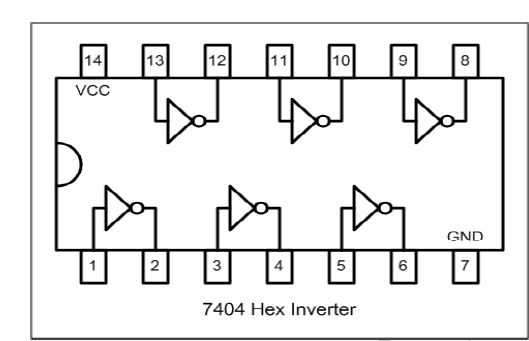
\includegraphics[width=0.6\linewidth, height = 5cm]{LAB-1/LAB-1.PNG}
           \caption{Pin diagram of the MM74C04}
       \end{figure}
      \item The DC transfer characteristics are determined by calculating the output voltage with varying the input voltage from 0V to 5V from a single inverter in the IC.  
       \begin{figure}[H]
          \centering
          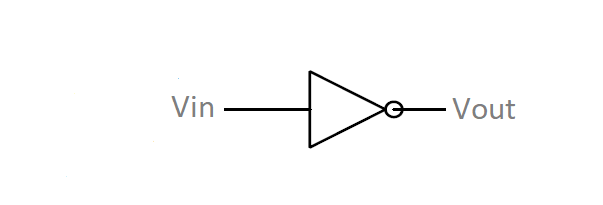
\includegraphics[width =0.5\linewidth]{LAB-1/LAB-1-i.PNG}
         \end{figure}
      \item The output characteristics is the variation of output voltage with output current, we measured output voltage VS output current via a potentiometer connected to the output terminal for two different cases a)Output is high b)Output is low 
        \begin{figure}[H]
          \centering
          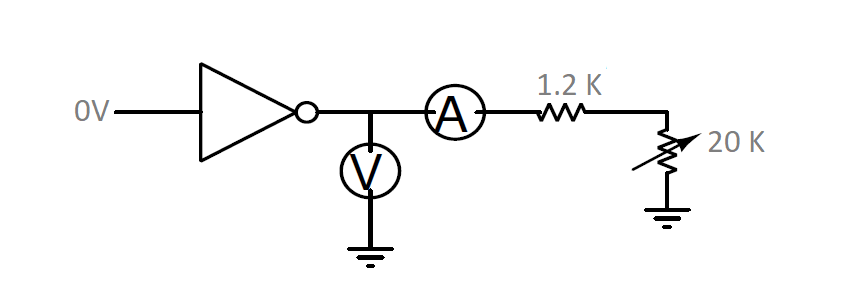
\includegraphics[width = 0.6\linewidth]{LAB-1/LAB-1-ii(a).PNG}
          \caption{Output characteristics when output is high}
        \end{figure}
        \begin{figure}[H]
          \centering
          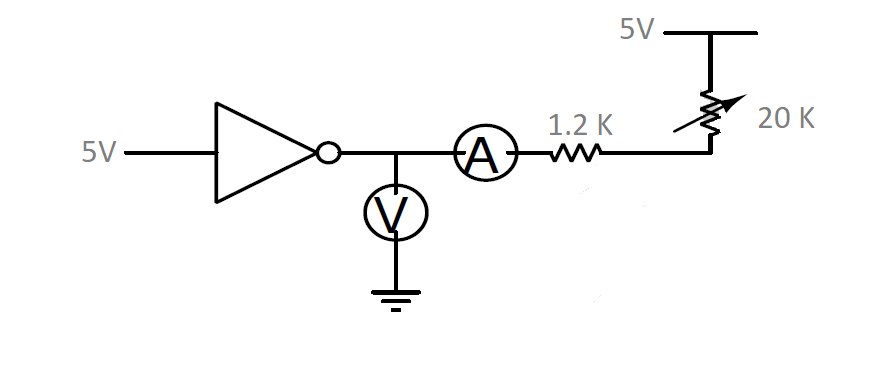
\includegraphics[width = 0.6\linewidth]{LAB-1/LAB-1-ii(b).PNG}
          \caption{Output characteristics when output is low}
        \end{figure}
      \item The delay of an inverter is measured using a \textbf{Ring Oscillator} which is a delay oscillator consisting of odd number of inverters  connected in a ring. The period of the oscillation is twice the sum of all the inverter delays. Also the delay depends on its load capacitance.
      \begin{equation}
          \ d = k_{0} + \tau_{inv}\frac{C_{load}}{C_{in}} \ (in \ seconds)
      \end{equation}
      $k_{0}$ is a constant and $\tau_{inv}$ is an inverter parameter
      delay(d) can be adjusted into $\tau_{inv}$ units and the equation becomes
            \begin{equation}
          d^* = p_{inv} + \frac{C_{load}}{C_{in}} \ (in \ \tau_{inv} \ units)
      \end{equation}
      \newpage
      We used 17 inverters in ring oscillator and calculated period(in s) of the oscillation for different loads(open inverters), the period is related to delay by
      \begin{equation}
          \tau \times (34p_{inv} + (32 + (2 \times (1 + AdditionalOutputLoad))))
      \end{equation}
      The Additional Output Load is the number of open inverters connected to the ring Oscillator
        \begin{figure}[H]
          \centering
          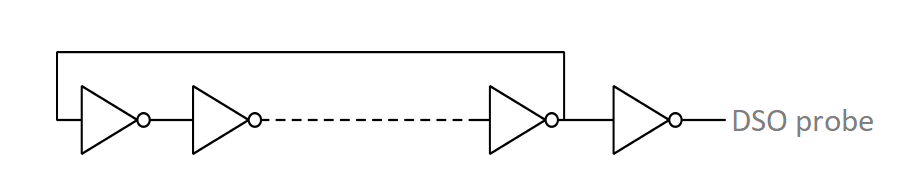
\includegraphics[width = 0.7\linewidth]{LAB-1/LAB-1-iii.PNG}
          \caption{Ring oscillator circuit with default load (=2)}
       \end{figure}
       \begin{figure}[H]
         \centering
         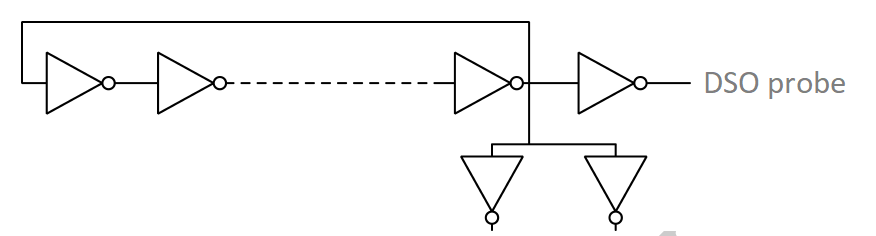
\includegraphics[width = 0.7\linewidth]{LAB-1/LAB-1-iii(b).PNG}
         \caption{Ring oscillator circuit with additional 3-inverter load}
       \end{figure}
    \item The delay of an inverter varies as the supply voltage is varied. We measured the ring oscillator period(to estimate the delay) for a fixed load(=2) at each voltage from 3V to 5V in 0.5 steps
       \begin{figure}[H]
         \centering
         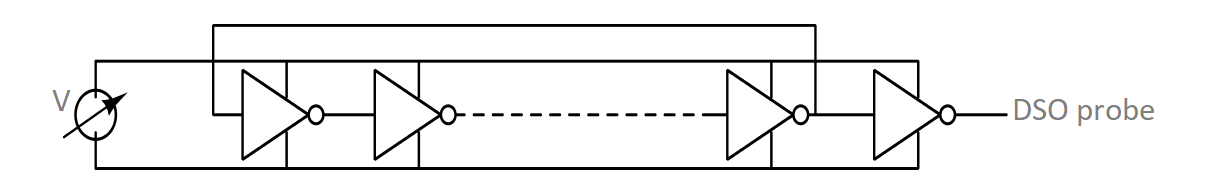
\includegraphics[width = 0.7\linewidth]{LAB-1/LAB-1-iv.PNG}
         \caption{Test circuit for measuring the delay as a function of supply voltage}
       \end{figure}
       \newpage
    \item Whenever an inverter output switches from low to high, current is drawn from the power supply. The current drawn is approximately a triangular pulse whose width is essentially the delay of the gate. We connected a resistor(R=1) in series with ground path to observe this. The voltage across the resistor is same as the current through it. 
       \begin{figure}[H]
         \centering
         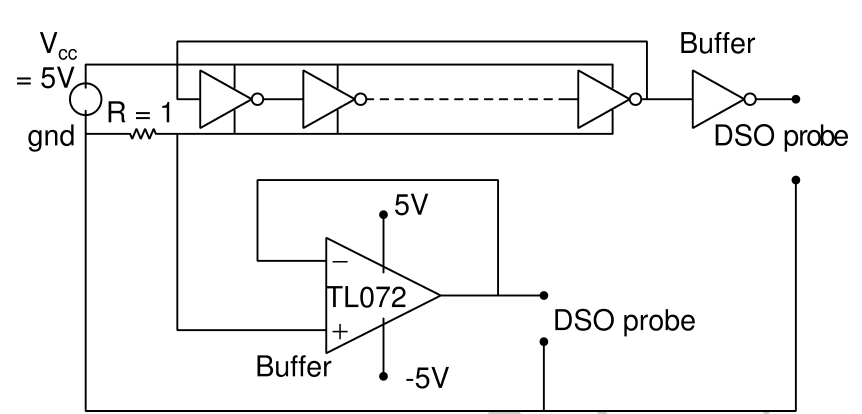
\includegraphics[width = 0.7\linewidth]{LAB-1/LAB-1-v.PNG}
         \caption{Circuit diagram for switching current measurement}
       \end{figure}
  \end{itemize}
  %\newpage
  
  %\vspace*{2pt}
  \section{Observations}
  \subsection{Transfer Characteristics}
  \begin{figure}[H]
    \begin{subfigure}{0.7\linewidth}
      \centering
      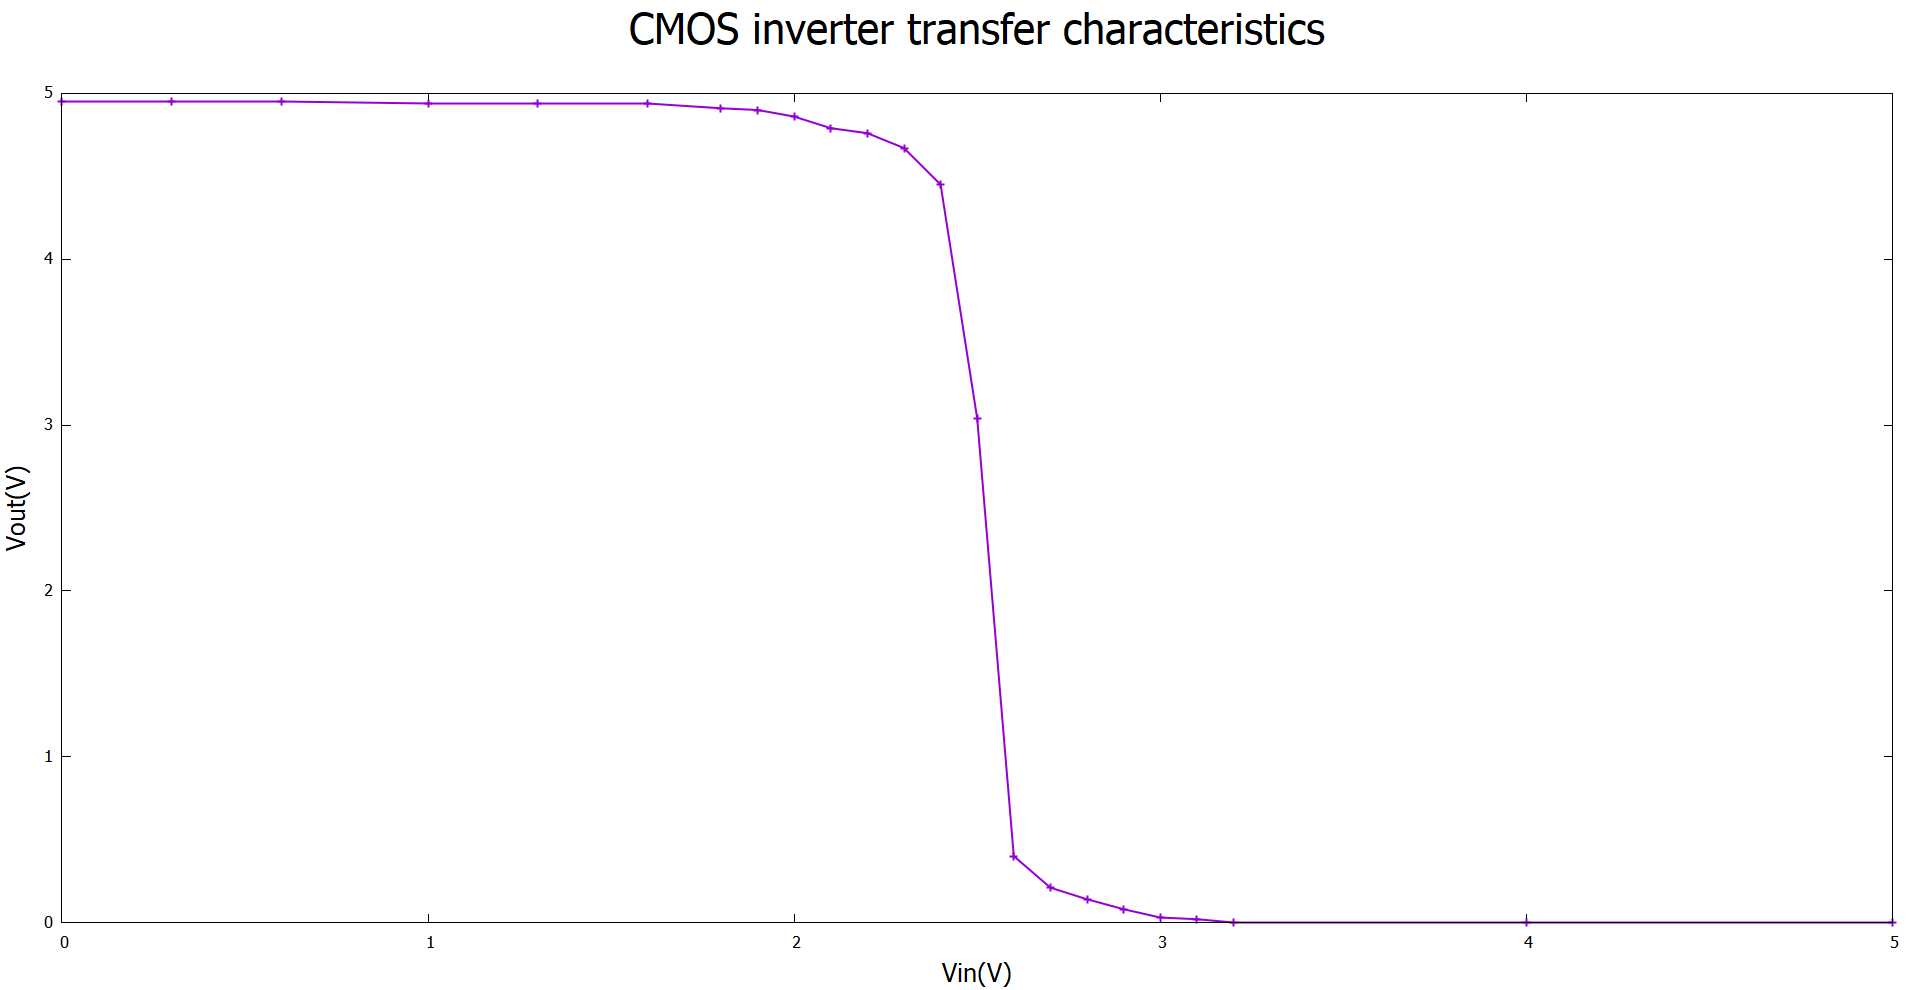
\includegraphics[width=\linewidth,height=4in]{LAB-1/LAB-1-1.png}
    \end{subfigure} 
    \begin{subfigure}{0.2\linewidth}
      \centering
      \begin{tabular}{|c|c|}
       \hline
       \bfseries $\mathbf{V_{in}}$	& \bfseries	$\mathbf{V_{out}}$	\\
       \hline
            0	&	4.95	\\
            0.3	&	4.95	\\
            0.6	&	4.95	\\
            1	&	4.94	\\
            1.3	&	4.94	\\
            1.6	&	4.94	\\
            1.8	&	4.91	\\
            1.9	&	4.9	    \\
            2	&	4.86	\\
            2.1	&	4.79	\\
            2.2	&	4.76	\\
            2.3	&	4.67	\\
            2.4	&	4.45	\\
            2.5	&	3.04	\\
            2.6	&	0.4	    \\
            2.7	&	0.21	\\
            2.8	&	0.14	\\
            2.9	&	0.08	\\
            3	&	0.03	\\
            3.1	&	0.02	\\
            3.2	&	0    	\\
            4	&	0   	\\
            5	&	0	    \\
           \hline
      \end{tabular}
    \end{subfigure} 
   \end{figure}

Therefore, from the graph we get that the switching point of CMOS inverter is around 2.5 V

\subsection{Output Characteristics}
\vspace{4mm}
  \begin{figure}[H]
    \begin{subfigure}{0.7\linewidth}
      \centering
      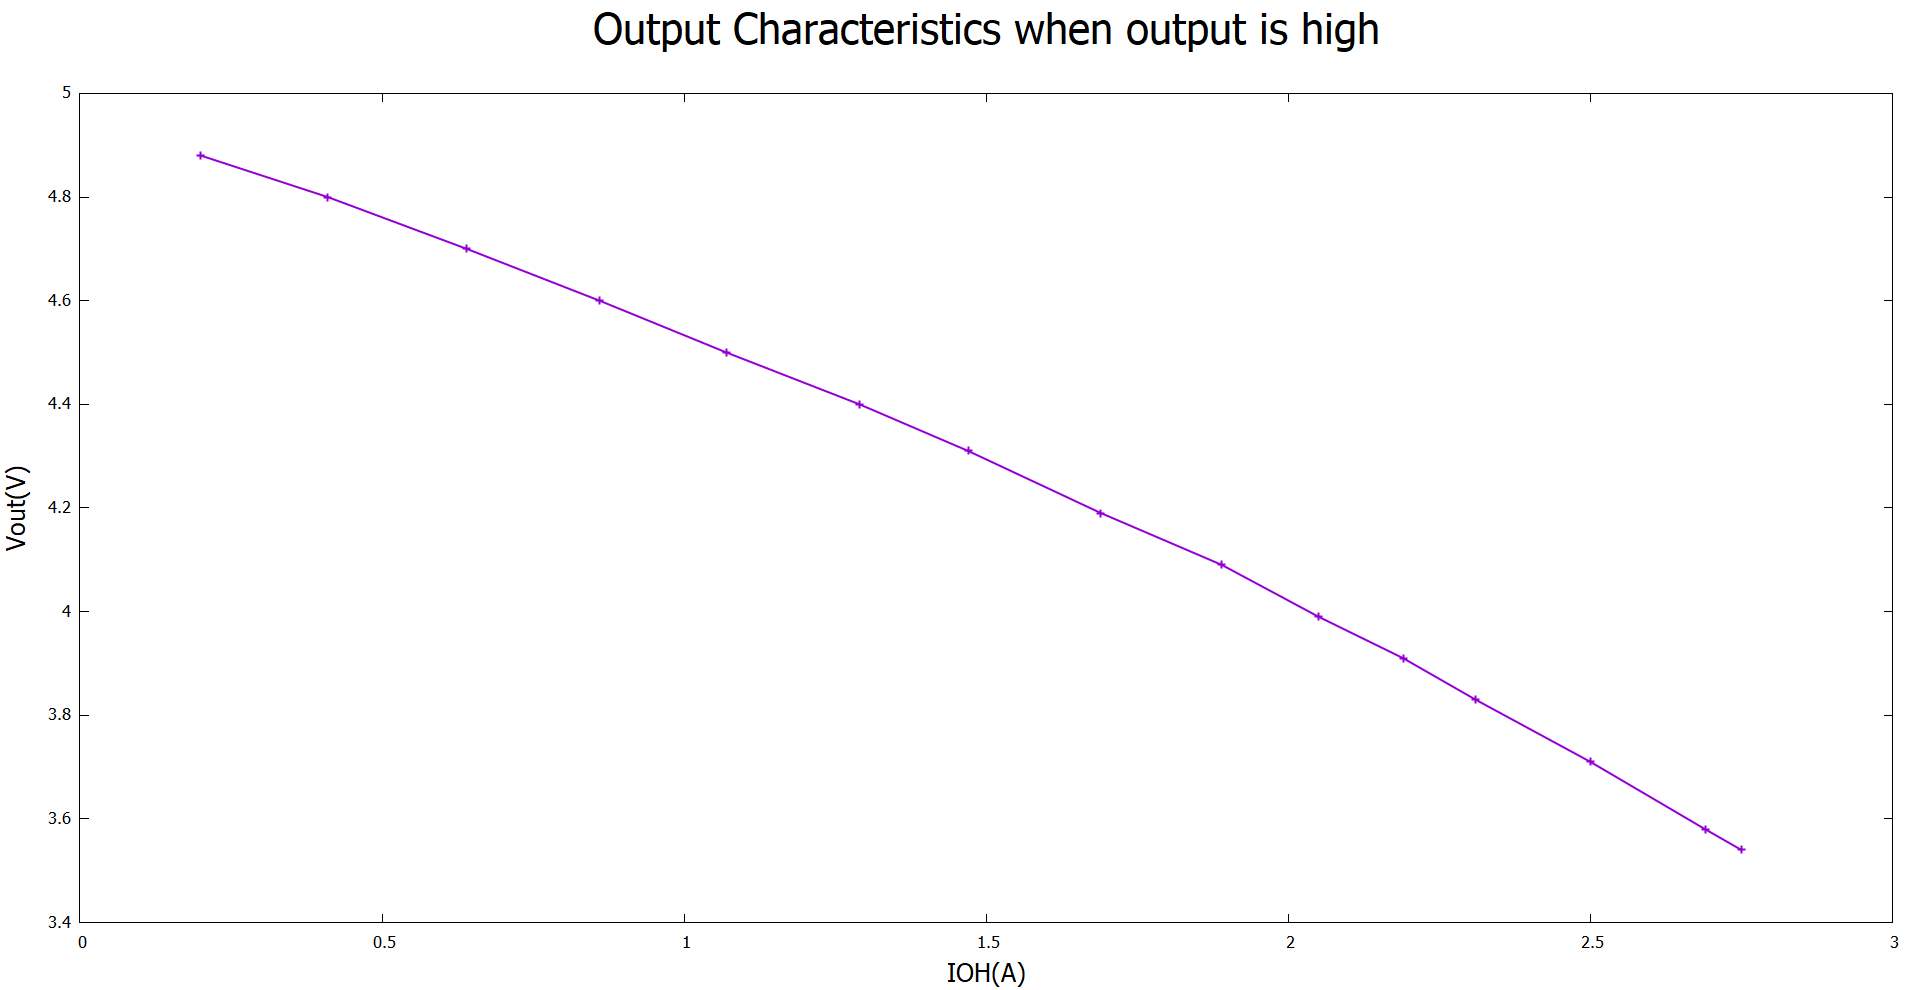
\includegraphics[width=\linewidth,height=3in]{LAB-1/LAB-1-2a.png}
    \end{subfigure} 
    \begin{subfigure}{0.2\linewidth}
      \centering
      \begin{tabular}{|c|c|}
       \hline
       \bfseries $\mathbf{V_{in}}$	& \bfseries	$\mathbf{V_{out}}$	\\
       \hline
            4.88 &	0.2        \\
            4.8	 &  0.41       \\
            4.7	 &  0.64       \\
            4.6	 &  0.86       \\
            4.5	 &  1.07       \\
            4.4	 &  1.29       \\     
            4.31 &	1.47       \\
            4.19 &	1.69       \\
            4.09 &	1.89        \\
            3.99 &	2.05      \\
            3.91 &	2.19      \\
            3.83 &	2.31          \\
            3.71 &	2.5          \\
            3.58 &	2.69       \\
            3.54 &	2.75          \\

           \hline
      \end{tabular}
    \end{subfigure} 
   \end{figure}
   
   \vspace{9mm}
   
   \begin{figure}[H]
    \begin{subfigure}{0.7\linewidth}
      \centering
      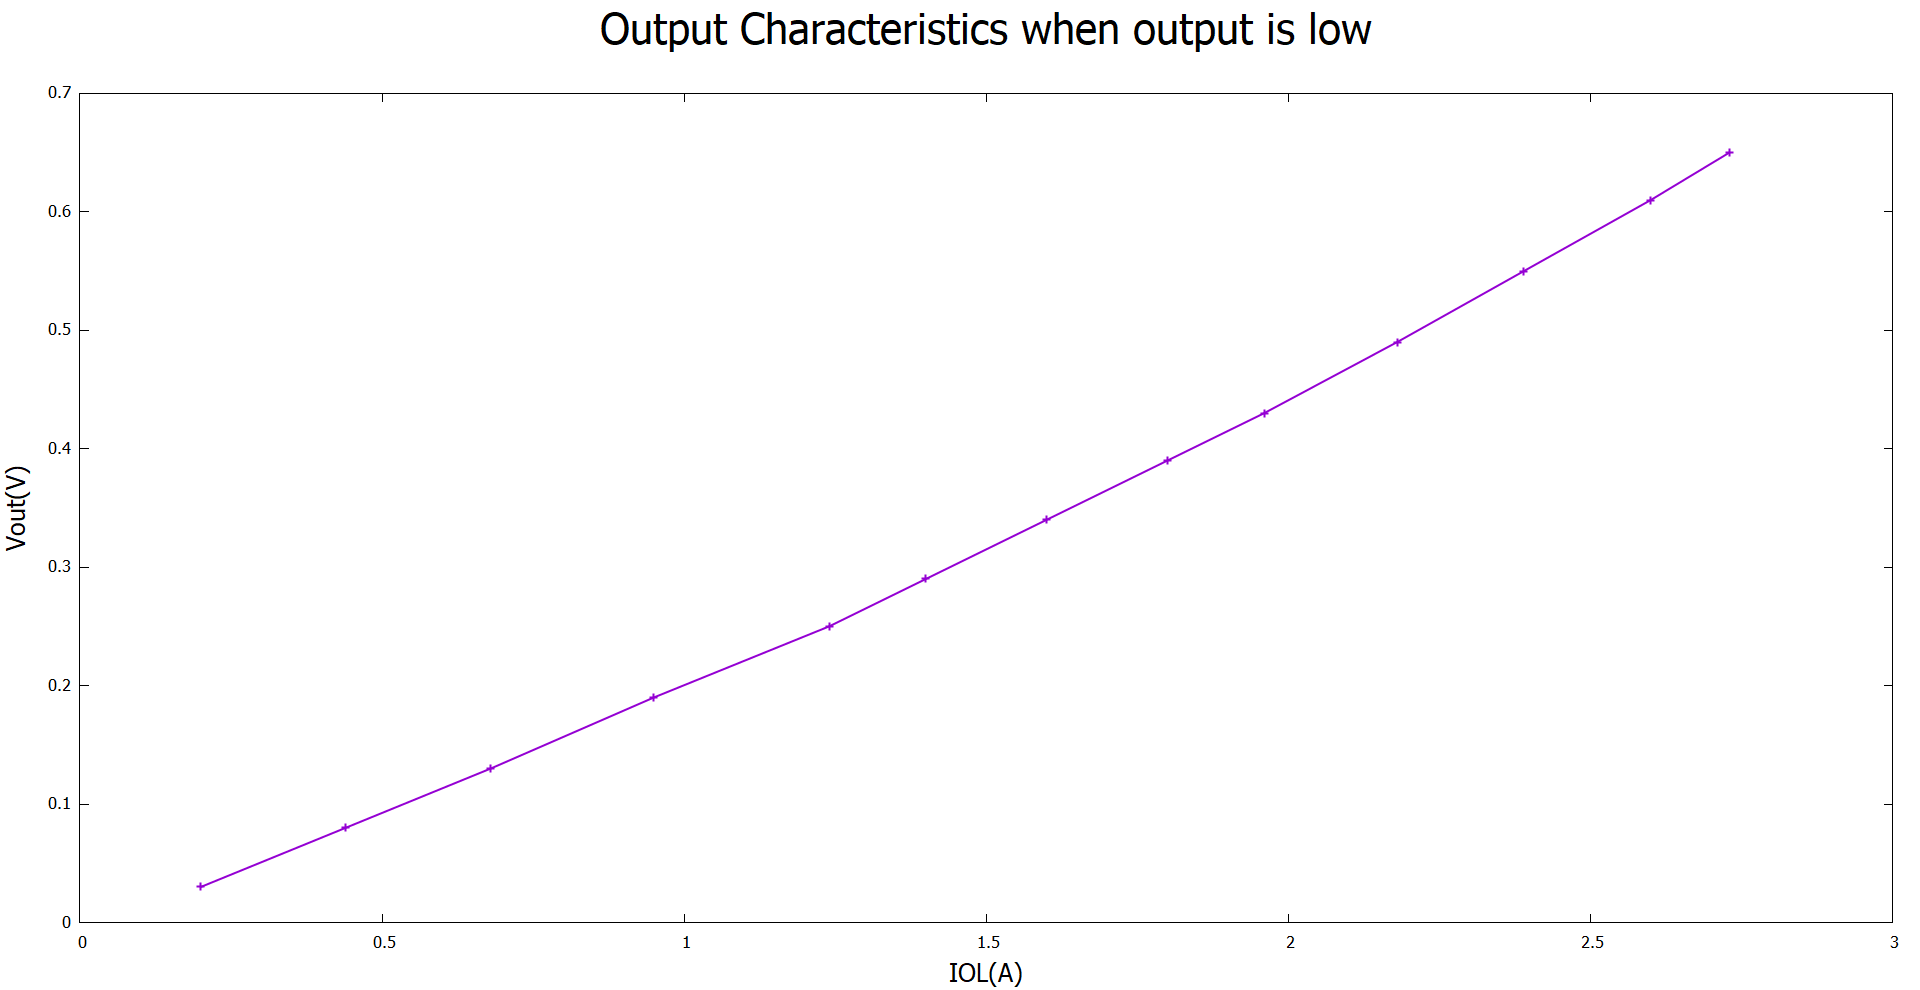
\includegraphics[width=\linewidth,height=3in]{LAB-1/LAB-1-2b.png}
    \end{subfigure} 
    \begin{subfigure}{0.2\linewidth}
      \centering
      \begin{tabular}{|c|c|}
       \hline
       \bfseries $\mathbf{V_{in}}$	& \bfseries	$\mathbf{V_{out}}$	\\
       \hline
            0.03 &	0.2\\
            0.08 &	0.44\\
            0.13 &	0.68\\
            0.19 &	0.95\\
            0.25 &	1.24\\
            0.29 &	1.4\\
            0.34 &	1.6\\
            0.39 &	1.8\\
            0.43 &	1.96\\
            0.49 &	2.18\\
            0.55 &	2.39\\
            0.61 &	2.6\\
            0.65 &	2.73\\

           \hline
      \end{tabular}
    \end{subfigure} 
   \end{figure}
   
\subsection{Delay of the Inverter}
\vspace{4mm}
  \begin{figure}[H]
    \begin{subfigure}{0.7\linewidth}
      \centering
      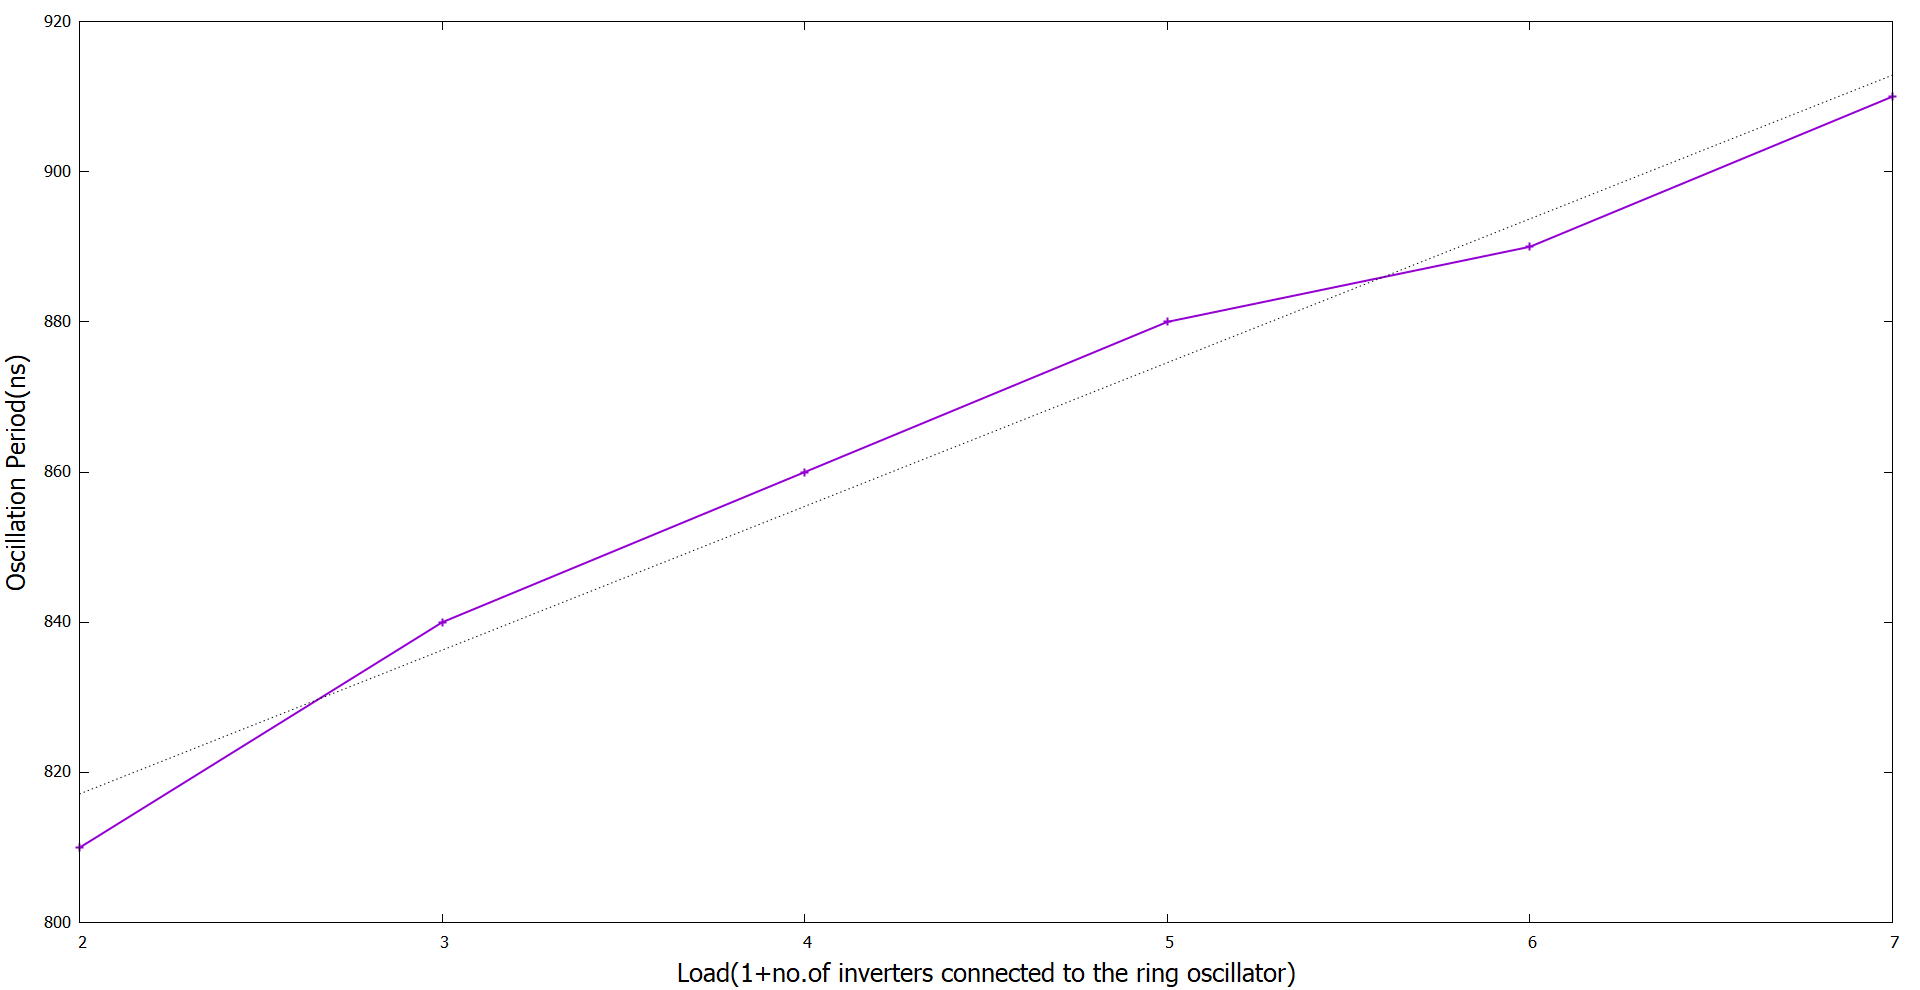
\includegraphics[width=\linewidth,height=2.5in]{LAB-1/LAB-1-3.png}
    \end{subfigure} 
    \begin{subfigure}{0.2\linewidth}
      \centering
      \begin{tabular}{|c|c|}
       \hline
       \bfseries Load	& \bfseries	Period(ns)	\\
       \hline
            2 &	810\\
            3 &	840\\
            4 &	860\\
            5 &	880\\
            6 &	890\\
            7 &	910\\
           \hline
      \end{tabular}
    \end{subfigure} 
   \end{figure}
   Slope and intercept of the best fit line are 19.14 n and 778.86 n respectively \\
   \\ 
    The period of the ring oscillator is given by:
    \vspace{4mm}
\begin{equation}
\tau \times (34p_{inv} + (32 + (2 \times (1 + AdditionalOutputLoad))))
\end{equation}
   measured in seconds.
\\
\\
    \vspace{1cm}
The slope of the above graph gives us $\tau_{inv} = 9.57 \ ns$, $p_{inv}$ comes out to be $1.39$
\begin{figure}[H]
    \centering
    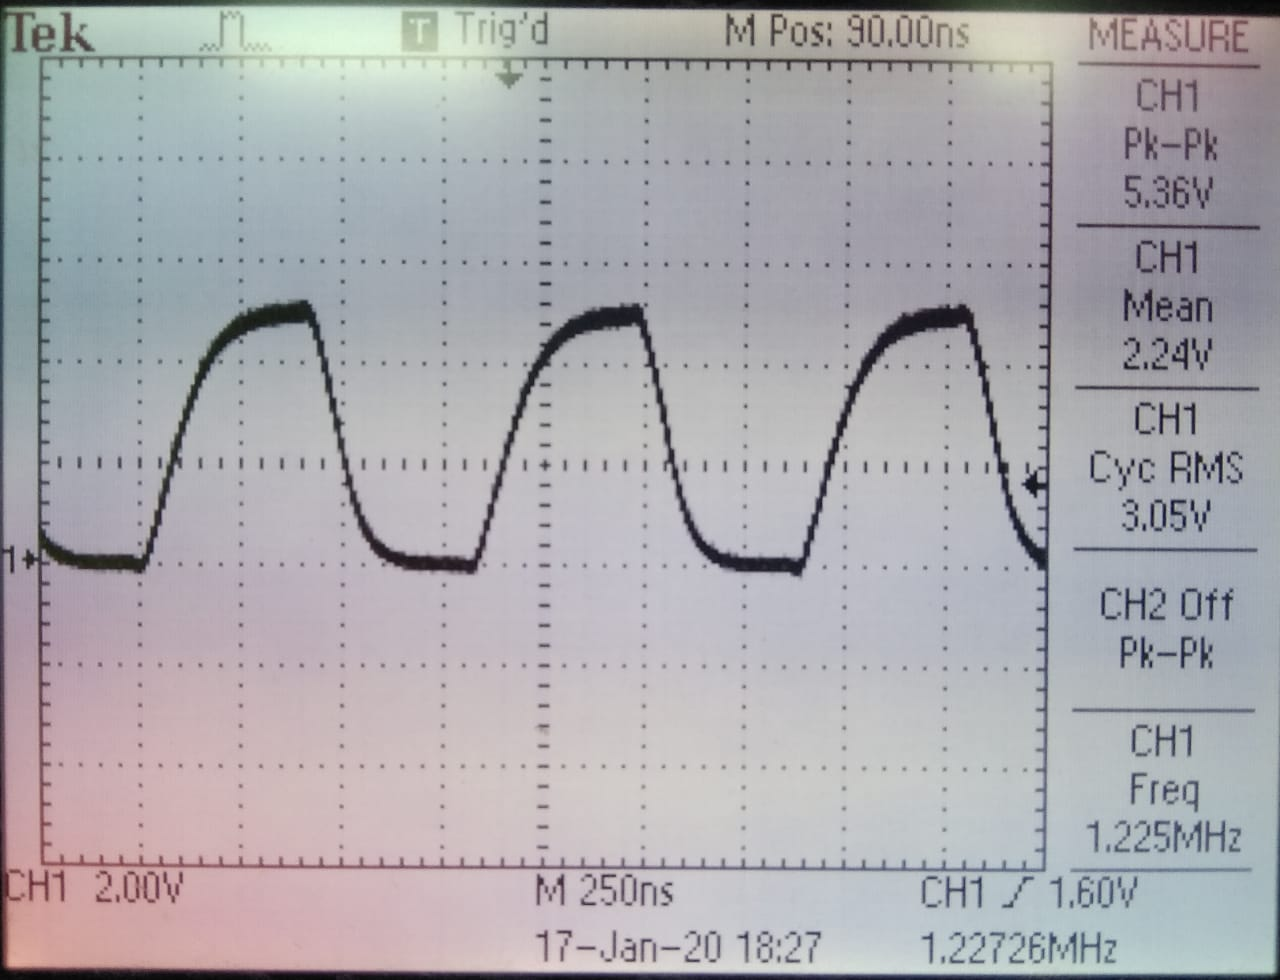
\includegraphics[width = 0.5\linewidth]{LAB-1/LAB-1-5V.jpeg}
    \caption{ring-oscillator output with load = 2}
\end{figure}
%\\
%\vspace{-4mm}
%The delay can be expressed in multiples of $\tau$ as
%\vspace{4mm}
%\begin{equation}
%d_{inv} = \rho_{inv} + \frac{C_{load}}{C_{in}}
%\end{equation}

%where $\rho_{inv} = \kappa_o / \tau$ is the parasitic delay of the inverter (measured in $\tau$ units).

%\vspace{4mm}
%From the graph, we get $\kappa_o = 778.86 $ ns. Therefore, $\rho_{inv}$ comes out to be $40.69$

\subsection{Dependence of Delay with supply voltage}
\vspace{4mm}
  \begin{figure}[H]
    \begin{subfigure}{0.7\linewidth}
      \centering
      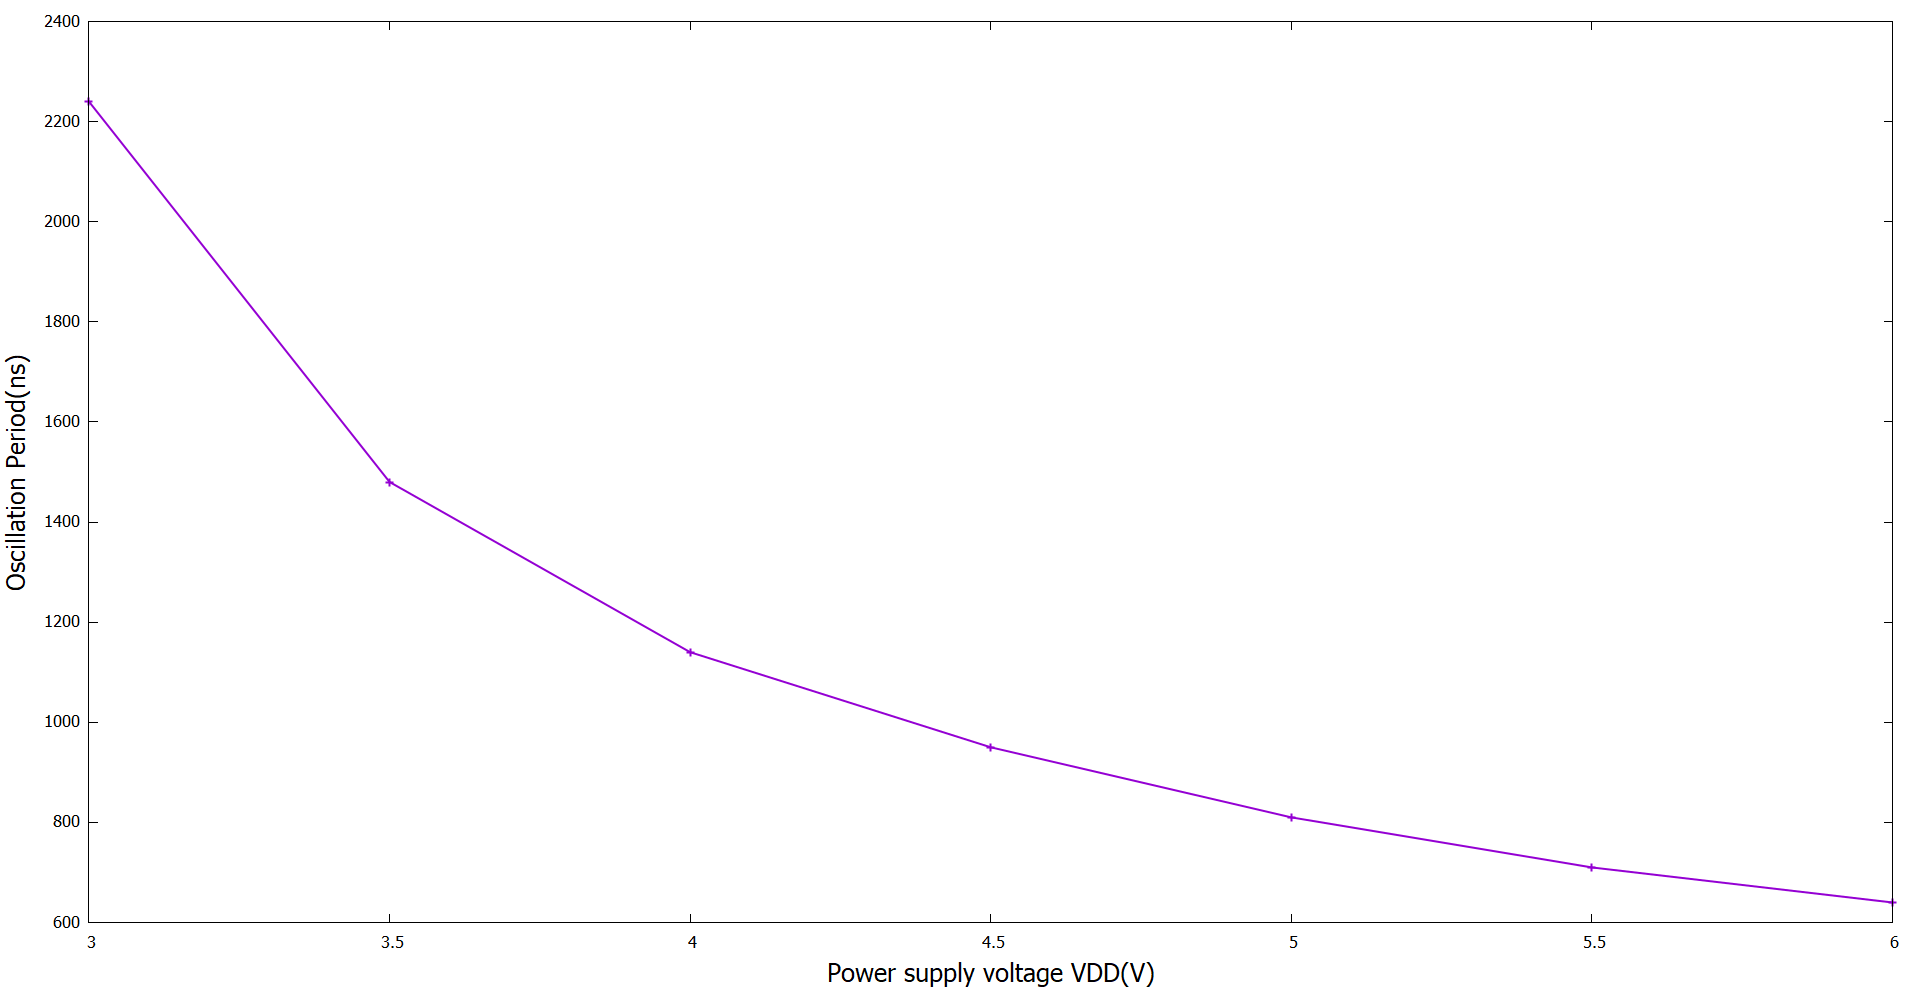
\includegraphics[width=\linewidth,height=2.6in]{LAB-1/LAB-1-4.png}
    \end{subfigure} 
    \begin{subfigure}{0.2\linewidth}
      \centering
      \begin{tabular}{|c|c|}
       \hline
       \bfseries $\mathbf{V_{DD}}$	& \bfseries	Period(ns)	\\
       \hline
            3 &	2240\\
            3.5 &	1480\\
            4 &	1140\\
            4.5 &	950\\
            5 &	810\\
            5.5 &	710\\
            6 &	640\\

        \hline
      \end{tabular}
    \end{subfigure}
   \end{figure}
   As evident from the plot, delay decreases with increase in power supply
   \begin{figure}[H]
     \begin{subfigure}{0.4\linewidth}
       \centering
       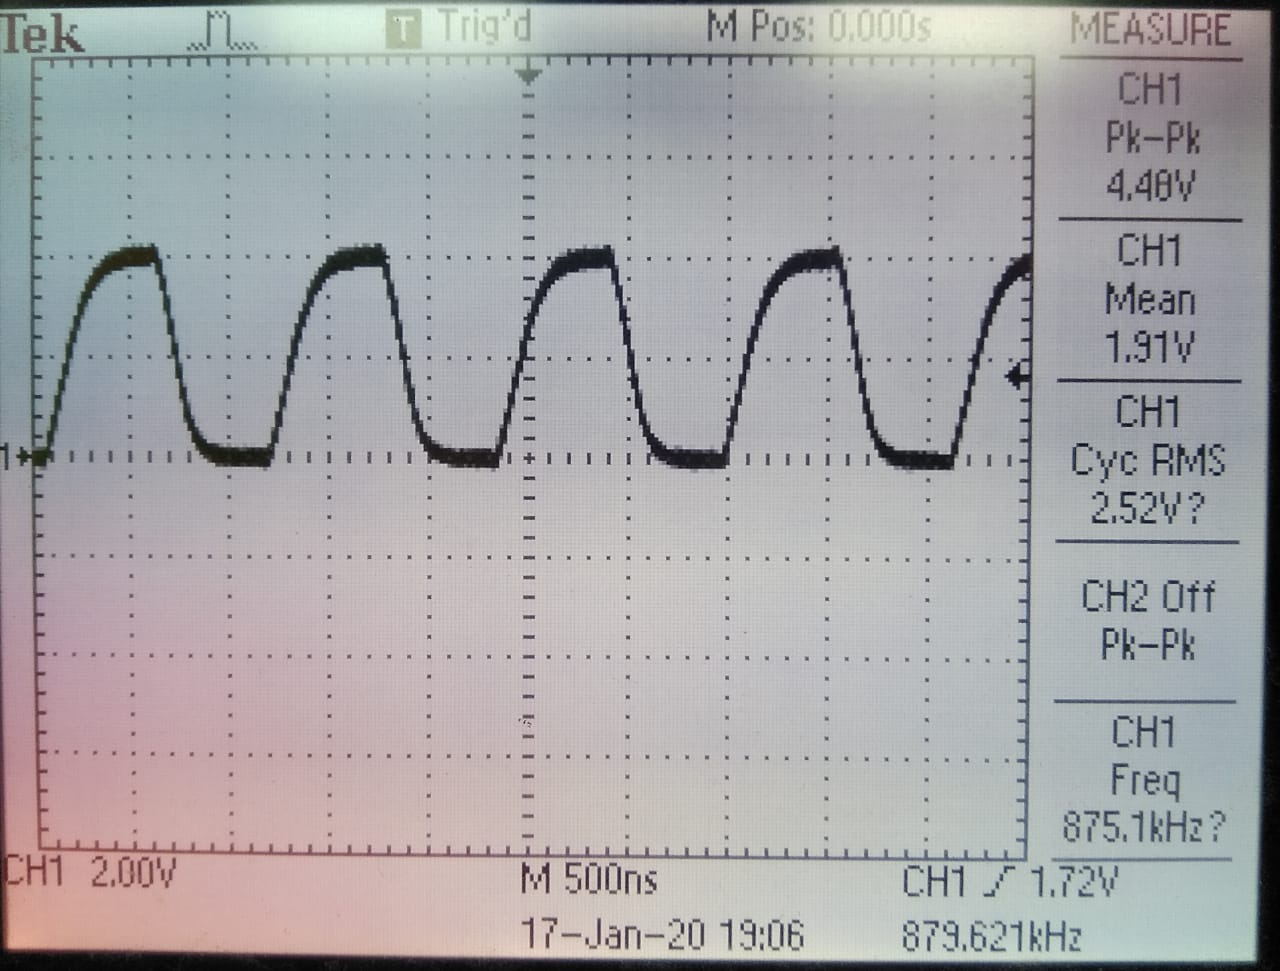
\includegraphics[width = \linewidth]{LAB-1/LAB-1-4V.jpeg}
       \caption{Ring-oscillator output at supply voltage = 4V }
     \end{subfigure}
     \begin{subfigure}{0.4\linewidth}
       \centering
       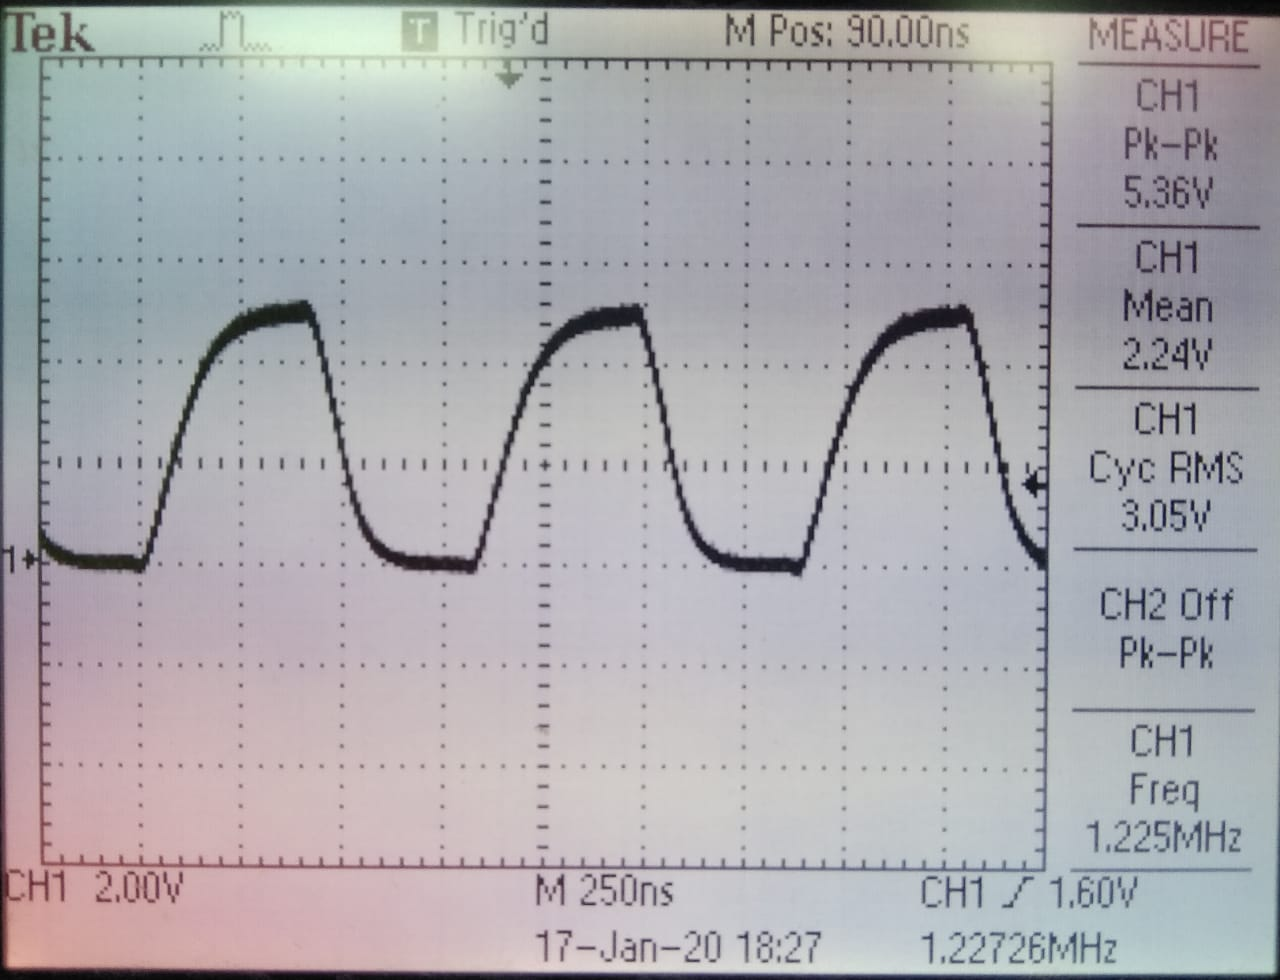
\includegraphics[width=\linewidth]{LAB-1/LAB-1-5V.jpeg}
       \caption{Ring-oscillator output at supply voltage = 5V}
     \end{subfigure}
   \end{figure}
   \begin{figure}[H]
       \centering
       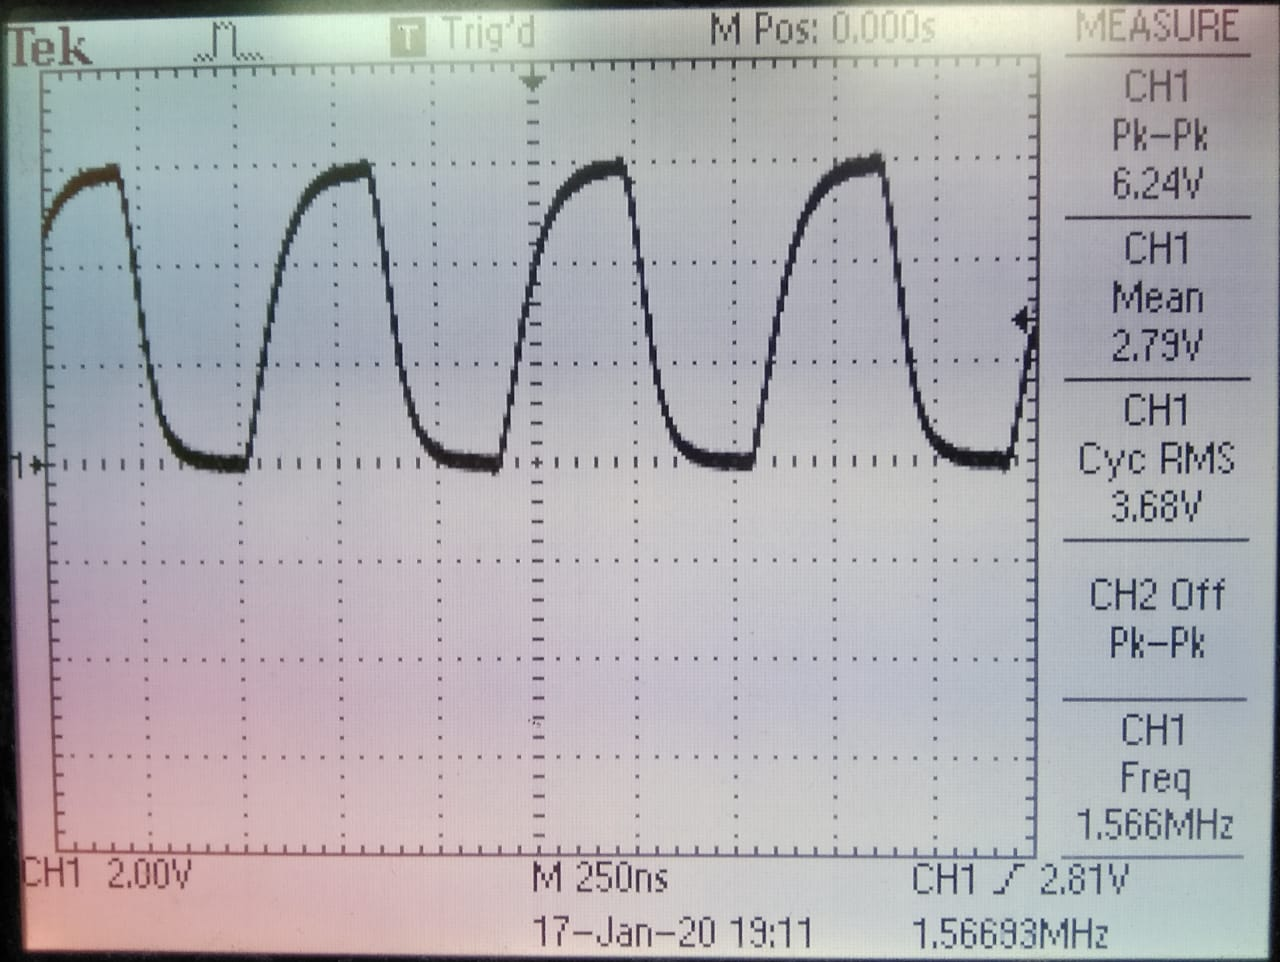
\includegraphics[width = 0.4\linewidth]{LAB-1/LAB-1-6V.jpeg}
       \caption{Ring-oscillator output at supply voltage = 6V}
   \end{figure}
   
   \subsection{Switching current through the power supply}
     
      \begin{figure}[H]
          \centering
          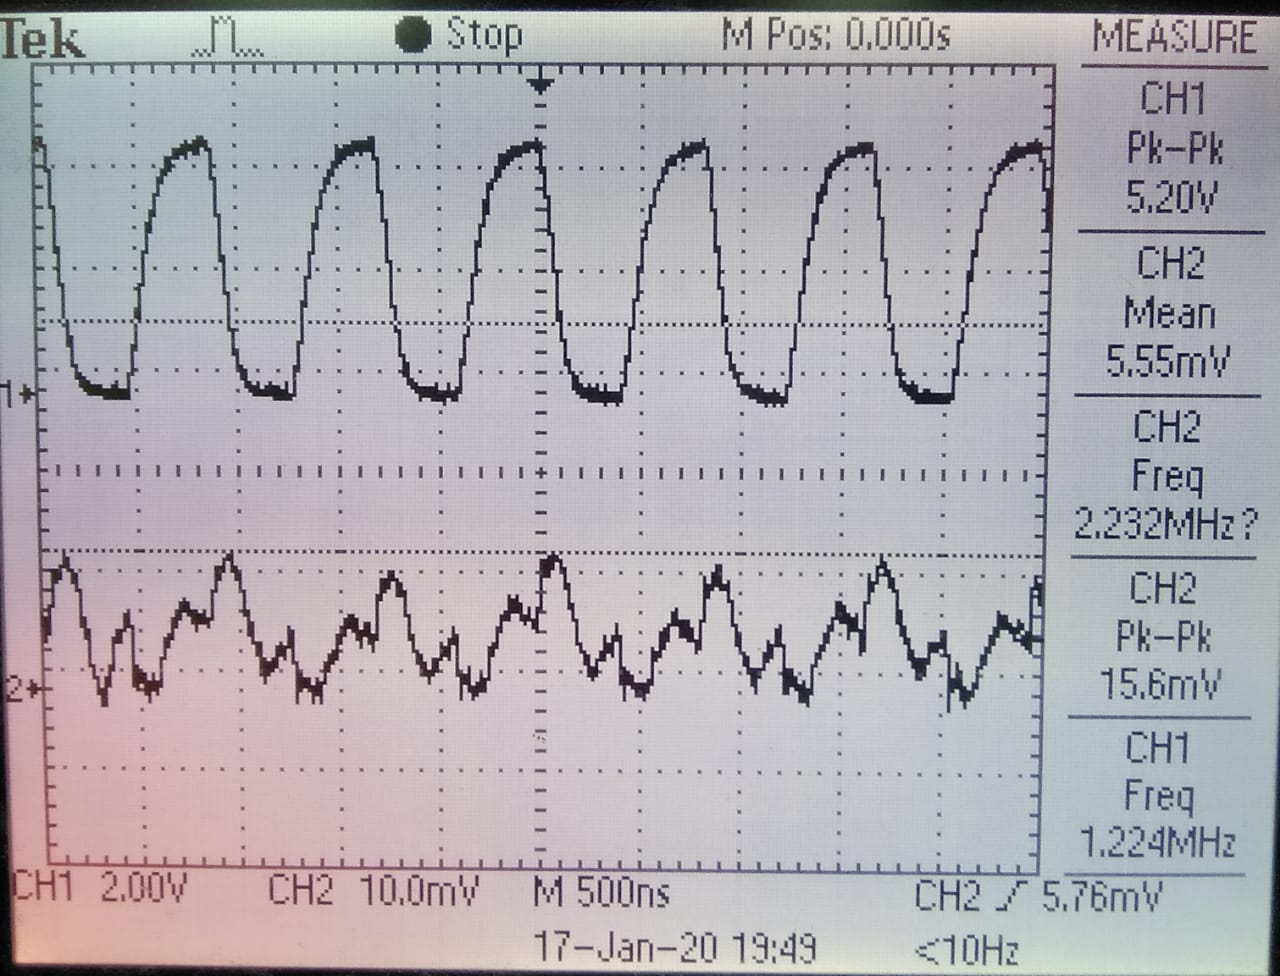
\includegraphics[width = 0.8\linewidth]{LAB-1/LAB-1-last.jpeg}
          \caption{ring-oscillator output and voltage across the 1$\Omega$ resistance}
      \end{figure}
      
      As evident from the figure, the average and peak value of switching current are $5.55mV$ and $15.6mV$ respectively.

\end{document}

